   
\documentclass[11pt]{article}
\renewcommand{\baselinestretch}{1.05}
\usepackage{amsmath,amsthm,verbatim,amssymb,amsfonts,amscd, graphicx}
\usepackage{mathtools}
\usepackage[table,xcdraw]{xcolor}
\DeclarePairedDelimiter{\ceil}{\lceil}{\rceil}
\usepackage{graphics}
\usepackage{enumitem}
\usepackage[table]{xcolor}
\usepackage{floatrow}
\usepackage{geometry}
\usepackage{tikz}
\usetikzlibrary{shapes.geometric,arrows,fit,matrix,positioning}
\tikzset
{
    treenode/.style = {rectangle, draw=black, align=center, minimum size=1cm},
    subtree/.style  = {isosceles triangle, draw=black, align=center, minimum height=0.5cm, minimum width=1cm, shape border rotate=90, anchor=north}
}
\topmargin0.0cm
\headheight0.0cm
\headsep0.0cm
\oddsidemargin0.0cm
\textheight23.0cm
\textwidth16.5cm
\footskip1.0cm
\theoremstyle{plain}
\newtheorem{theorem}{Theorem}
\newtheorem{corollary}{Corollary}
\usepackage{clrscode}
\newtheorem{lemma}{Lemma}
\newtheorem{proposition}{Proposition}
\newtheorem*{surfacecor}{Corollary 1}
\newtheorem{conjecture}{Conjecture} 
\newtheorem{question}{Question} 
\theoremstyle{definition}
\newtheorem{definition}{Definition}

\newlist{pcases}{enumerate}{1}
\setlist[pcases]{
  label=\underline{Case~\arabic*:}\protect\thiscase.~,
  ref=\arabic*,
  align=left,
  labelsep=0pt,
  leftmargin=0pt,
  labelwidth=0pt,
  parsep=0pt
}
\newcommand{\case}[1][]{%
  \if\relax\detokenize{#1}\relax
    \def\thiscase{}%
  \else
    \def\thiscase{~#1}%
  \fi
  \item
}
\usepackage{listings}
\usepackage{color}

\definecolor{dkgreen}{rgb}{0,0.6,0}
\definecolor{gray}{rgb}{0.5,0.5,0.5}
\definecolor{mauve}{rgb}{0.58,0,0.82}

\lstset{frame=tb,
  language=Java,
  aboveskip=3mm,
  belowskip=3mm,
  showstringspaces=false,
  columns=flexible,
  basicstyle={\small\ttfamily},
  numbers=none,
  numberstyle=\tiny\color{gray},
  keywordstyle=\color{blue},
  commentstyle=\color{dkgreen},
  stringstyle=\color{mauve},
  breaklines=true,
  breakatwhitespace=true
  tabsize=3
}
\newcommand{\blank}[1]{\hfil\penalty1000\hfilneg\rule[-3pt]{#1}{0.4pt}}
\begin{document}
 


\title{Fun with Trees (no, not binary trees)}
\author{By Joshua Kirstein (joshkirstein@ufl.edu)}
\maketitle

\section{Introduction}
In this set of lecture notes we're going to take a close look at trees. Right now you're probably thinking about binary trees, binary search trees, balanced binary search trees, etc. While these are trees, they're a very specific type of tree. In the notation we'll develop, a binary tree is a \emph{rooted} tree in which each node is allowed at most two children. In general, however, trees are not rooted (keep in mind that in this case the term \emph{child} does not make much sense). We'll be covering general trees as well as rooted trees.
\section{Definitions}
Before we begin there needs to be a clarification about what we're talking about. There are actually many \emph{equivalent} definitions of trees, meaning that they're different ways of talking about the same thing. Certain definitions are easier to use in different situations, but we'll mention the three most relevant ones.
\\\\
A \emph{tree} is an undirected, unweighted graph $G$ that satisfies any one of the following three conditions:
\\\\
(1) $G$ is connected and contains $V-1$ edges ($V$ is the number of vertices in $G$) \\
(2) $G$ is connected and is acyclic (contains no cycles) \\
(3) There is one unique path between any pair of nodes in $G$
\\\\
Because all of these conditions are equivalent, if one of them is true then so are the rest. Again, \emph{any} of these definitions are perfectly valid for a tree and in some cases one may be more useful than the others.
\begin{figure}[!ht]
\caption{An example (unrooted) tree.}
\centering
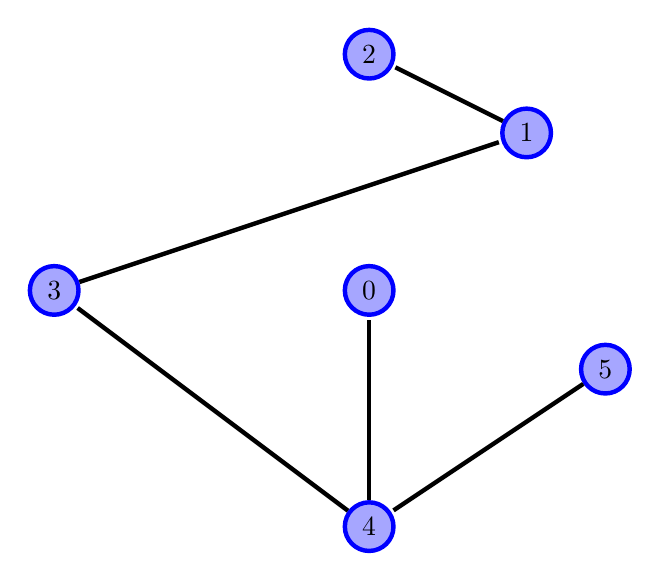
\begin{tikzpicture}[shorten >=1pt, auto, node distance=3cm, ultra thick]
   \begin{scope}[every node/.style={circle,draw=blue,fill=blue!35!}]
    \node (v1) at (0,0) {0};
    \node (v2) at (2, 2) {1};
    \node (v3) at (0, 3) {2};
    \node (v4) at (-4, 0) {3};
    \node (v5) at (0, -3) {4};
    \node (v6) at (3, -1) {5};
   \end{scope}
   \begin{scope}[every edge/.style={draw=black,ultra thick}]
    \draw  (v2) edge node{} (v3);
    \draw  (v5) edge node{} (v4);
    \draw  (v6) edge node{} (v5);
    \draw  (v5) edge node{} (v1);
    \draw  (v4) edge node{} (v2);
   \end{scope}
\end{tikzpicture}
\end{figure}
\newpage
\noindent
Please verify that each one of the conditions (1) - (3) are satisfied for the tree above. Notice how this tree doesn't really look like what traditional trees look like (you know when you draw them level-by-level with a root).
\\\\
In addition to trees, we'll be encountering rooted trees. A \emph{rooted} tree is a tree that is imbued with a specific node called the \emph{root}. Typically, rooted trees are drawn starting from the root at the top, growing downward. The definitions of \emph{parent} and \emph{child} nodes are the same in rooted trees as in binary trees, except parents may have more than two children.
\begin{figure}[!ht]
\caption{An example rooted tree. The node labelled `r' is the root.}
\centering
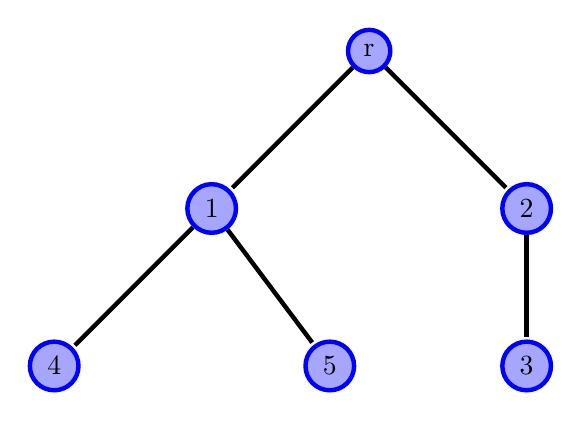
\begin{tikzpicture}[shorten >=1pt, auto, node distance=3cm, ultra thick]
   \begin{scope}[every node/.style={circle,draw=blue,fill=blue!35!}]
    \node (v1) at (0,0) {r};
    \node (v2) at (-2, -2) {1};
    \node (v3) at (2, -2) {2};
    \node (v4) at (2, -4) {3};
    \node (v5) at (-4, -4) {4};
    \node (v6) at (-0.5, -4) {5};
   \end{scope}
   \begin{scope}[every edge/.style={draw=black,ultra thick}]
    \draw  (v1) edge node{} (v2);
    \draw  (v1) edge node{} (v3);
    \draw  (v2) edge node{} (v5);
    \draw  (v2) edge node{} (v6);
    \draw  (v3) edge node{} (v4);
   \end{scope}
\end{tikzpicture}
\end{figure}
\\
The figure above pictures a rooted tree. Please verify that all of the regular conditions that a tree must satisfy are satisfied, as well as observe the fact that there is a root (labelled `r' in this example).
\section{Representing Trees in Memory}
Before we dive into algorithms related to trees, we first need to develop a method to store trees programmatically. We'll handle regular trees and rooted trees differently.
\subsection{Regular Trees}
A regular tree can be stored in the exact same ways as any ordinary graph. One important thing to keep in mind is that each tree contains \emph{exactly} $V-1$ edges, and thus it doesn't make sense to use an adjacency matrix to store it (since an adjacency matrix has enough storage for $V^2$ edges). Therefore, we will use an adjacency list to store a tree instead. We assume the nodes are labelled $0$ to $n-1$.
\begin{lstlisting}
//initialize adjacency list
ArrayList[] adj_list = new ArrayList[n];
for (int i = 0; i < n; i++)
	adj_list[i] = new ArrayList();
//read in the edges (there are n-1 of them *ALWAYS*)
for (int i = 0; i < (n-1); i++) {
	int from = readInt();
	int to = readInt();
	adj_list[from].add(to);
	adj_list[to].add(from);
}
//....use the adjacency list
\end{lstlisting}
\subsection{Rooted Trees}
Our code for representing rooted trees will be nearly identical to that of the regular tree, except for one slight modification. With rooted trees, it's often important to know the parent of each node and so after we're given the edges of the rooted tree as well as the root, we will have to go ahead and compute the parents for each node. How can we compute the parents of each node? By definition, the parent of a node is the \emph{first} node we encounter on our way up to the root from that node (in other words, the node right above). We'll use a depth-first search starting from the root and working our way down to each node. 
\begin{lstlisting}
//initialize adjacency list
ArrayList[] adj_list = new ArrayList[n];
for (int i = 0; i < n; i++)
	adj_list[i] = new ArrayList();
//read in the edges (there are n-1 of them *ALWAYS*)
for (int i = 0; i < (n-1); i++) {
	int from = readInt();
	int to = readInt();
	adj_list[from].add(to);
	adj_list[to].add(from);
}
//read root
int root = readInt();
//initialize parent array
int[] parent = new int[n];
//initialize level array
//level[node] = number of edges from the root to `node'
int[] level = new int[n];

//fill in parents array by using a dfs
//root is the very top, so -1 indicates
//that the root doesn't have a previous node (read: parent)
level[root] = 0;
dfs(root, -1);

void dfs(int current_node, int previous_node) {
	//the parent of the current node
	//is the node we just came from in the dfs
	//down from the root (by definition)
	parent[current_node] = previous_node;
	//compute the level for all non-root nodes
	if (previous_node != -1)
		level[current_node] = level[previous_node] + 1;
	//go through each node adjacent to the current
	//and call dfs on it
	for (int adjacent_node : adj_list[current_node]) {
		//we don't want to go back up, from where we just
		//came, so we skip `previous_node'
		if (adjacent_node == previous_node) continue;
		//move on to the next node down,
		//making the previous node equal to the current
		dfs(adjacent_node, current_node);
	}
}
\end{lstlisting}
Notice how this code is also computing the `level[]' array which we didn't talk about above. This is just another useful quantity we want to know for each node; refer to the code for what the definition of the level of a node is, as well as how to compute it.
\\\\
There's one last important thing to notice. In a traditional depth-first search we keep a `visited[]' array that tells us when a node is visited so that we don't end up in a recursive infinite loop. In the code above there is no `visited[]' array --- shouldn't this be a problem? Well actually we just replaced the `visited[]' array with another equivalent way of preventing infinite recursion: in trees, since there are no cycles, all we need to do is make sure we don't DFS back from where we came from and so it's sufficient to just ignore the previous node (our parent). If you are not convinced, try and step through the algorithm yourself on the rooted tree example above.
\section{Lowest Common Ancestor on Rooted Trees}
Suppose we are given a rooted tree. We define the \emph{lowest common ancestor} of two nodes $u$ and $v$, denoted $LCA(u, v)$, as the lowest node that is common to both node-to-root paths (a node-to-root path is the path from a node up to the root). Our goal is to compute $LCA(u, v)$ as quickly as possible for any nodes $u$ and $v$. You may notice that this seems a whole lot like a query problem; the $LCA(u, v)$ function \emph{is} a query on the tree given. In some of the solutions provided, we will need to precompute some data ahead of time in order to speed up the query time --- a theme that is prevalent in most query problems.
\subsection{The Easy Way (two pointer method)}
Take a minute and try to figure out how to compute the lowest common ancestor of two nodes. Any ideas? Take a look at the following tree (annotated with the levels of the tree) and try to compute $LCA(6, 5)$.
\begin{figure}[!ht]
\caption{$LCA(6, 5) = 1$.}
\centering
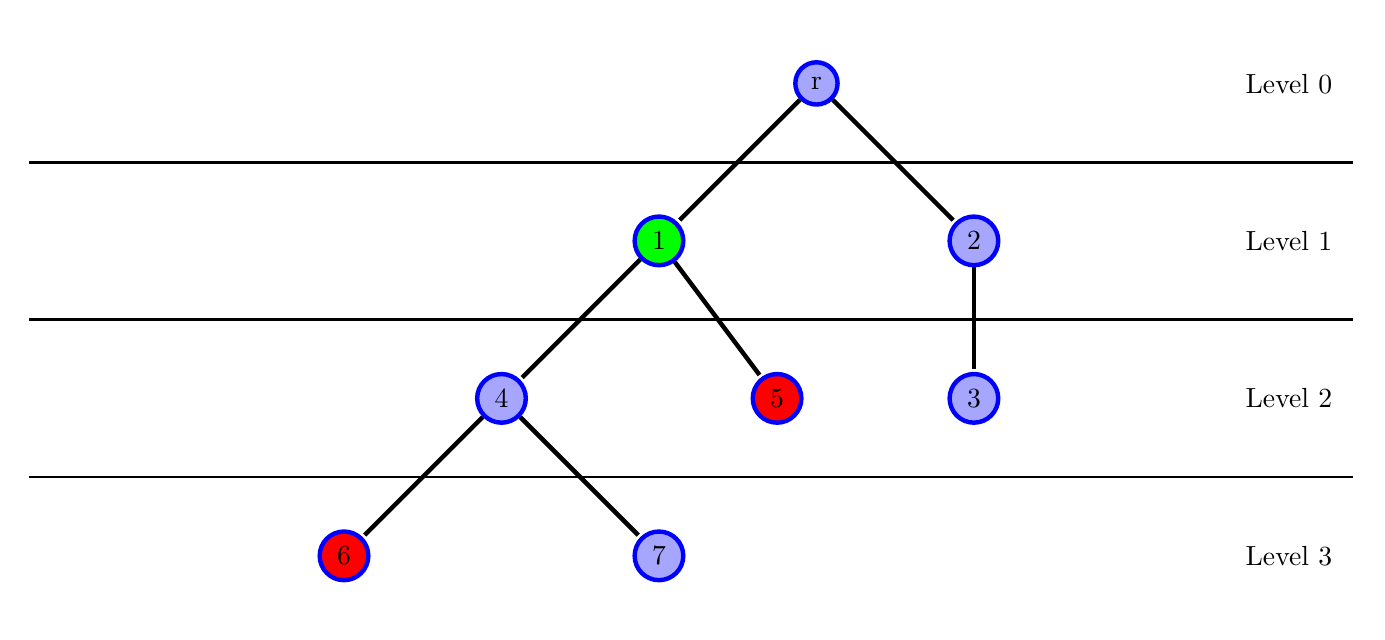
\begin{tikzpicture}[shorten >=1pt, auto, node distance=3cm, ultra thick]
   \node[circle] at (6,0) {{Level 0}};
   \node[circle] at (6,-2) {{Level 1}};
   \node[circle] at (6,-4) {{Level 2}};
   \node[circle] at (6,-6) {{Level 3}};
   \draw (-10,-1) -- (6.85,-1) [line width=1.0pt];
   \draw (-10,-3) -- (6.85,-3) [line width=1.0pt];
   \draw (-10,-5) -- (6.85,-5) [line width=1.0pt];
   \begin{scope}[every node/.style={circle,draw=blue,fill=blue!35!}]
    \node (v1) at (0,0) {r};
    \node (v2) at (-2, -2) [fill=green] {1};
    \node (v3) at (2, -2) {2};
    \node (v4) at (2, -4) {3};
    \node (v5) at (-4, -4) {4};
    \node (v6) at (-0.5, -4) [fill=red] {5};
    \node (v7) at (-6, -6) [fill=red] {6};
    \node (v8) at (-2, -6) {7};
   \end{scope}
   \begin{scope}[every edge/.style={draw=black,ultra thick}]
    \draw  (v1) edge node{} (v2);
    \draw  (v1) edge node{} (v3);
    \draw  (v2) edge node{} (v5);
    \draw  (v2) edge node{} (v6);
    \draw  (v3) edge node{} (v4);
    \draw  (v5) edge node{} (v7);
    \draw  (v5) edge node{} (v8);
   \end{scope}
   %\draw (-7.5,-8) edge [->, orange] node{} (v7);
   %\draw (1.3, -4.3) edge [->, orange] node{} (v6);
\end{tikzpicture}
\end{figure}
There are many ways to algorithmically calculate the LCA of two nodes. We can follow each node upward to the root, marking each node as visited along the way, and choose the first node that is visited on the other node's path to the root. This requires $O(n)$ memory to store the visited array and an $O(n)$ loop to clear the visited array after each run.
\\\\
\noindent
A more efficient solution is the \emph{two pointer method} which utilizes the `level[]' array to compute the LCA. The basic idea is to have two pointers, initially starting on the query nodes, and gradually we'll move them up the tree until they meet --- at this point, they should both be on the LCA.
\begin{figure}[!ht]
\caption{Initialize the pointers to start on the query nodes.}
\centering
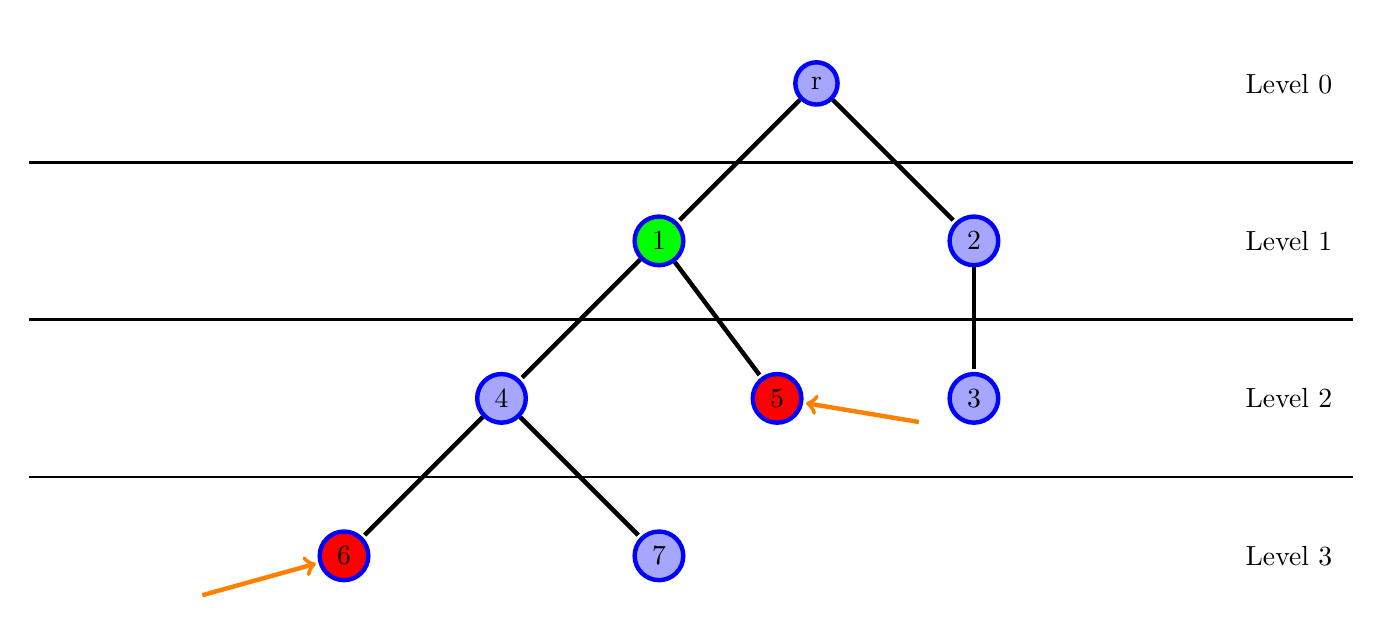
\begin{tikzpicture}[shorten >=1pt, auto, node distance=3cm, ultra thick]
   \node[circle] at (6,0) {{Level 0}};
   \node[circle] at (6,-2) {{Level 1}};
   \node[circle] at (6,-4) {{Level 2}};
   \node[circle] at (6,-6) {{Level 3}};
   \draw (-10,-1) -- (6.85,-1) [line width=1.0pt];
   \draw (-10,-3) -- (6.85,-3) [line width=1.0pt];
   \draw (-10,-5) -- (6.85,-5) [line width=1.0pt];
   \begin{scope}[every node/.style={circle,draw=blue,fill=blue!35!}]
    \node (v1) at (0,0) {r};
    \node (v2) at (-2, -2) [fill=green] {1};
    \node (v3) at (2, -2) {2};
    \node (v4) at (2, -4) {3};
    \node (v5) at (-4, -4) {4};
    \node (v6) at (-0.5, -4) [fill=red] {5};
    \node (v7) at (-6, -6) [fill=red] {6};
    \node (v8) at (-2, -6) {7};
   \end{scope}
   \begin{scope}[every edge/.style={draw=black,ultra thick}]
    \draw  (v1) edge node{} (v2);
    \draw  (v1) edge node{} (v3);
    \draw  (v2) edge node{} (v5);
    \draw  (v2) edge node{} (v6);
    \draw  (v3) edge node{} (v4);
    \draw  (v5) edge node{} (v7);
    \draw  (v5) edge node{} (v8);
   \end{scope}
   \draw (-7.8,-6.5) edge [->, orange] node{} (v7);
   \draw (1.3, -4.3) edge [->, orange] node{} (v6);
\end{tikzpicture}
\end{figure}
\newpage
\noindent
The first step is to bring both pointers to the same level. To do this, we simply move the lowest pointer up until both are on the same level.
\begin{figure}[!ht]
\caption{Move the lowest pointer upward until both are on the same level.}
\centering
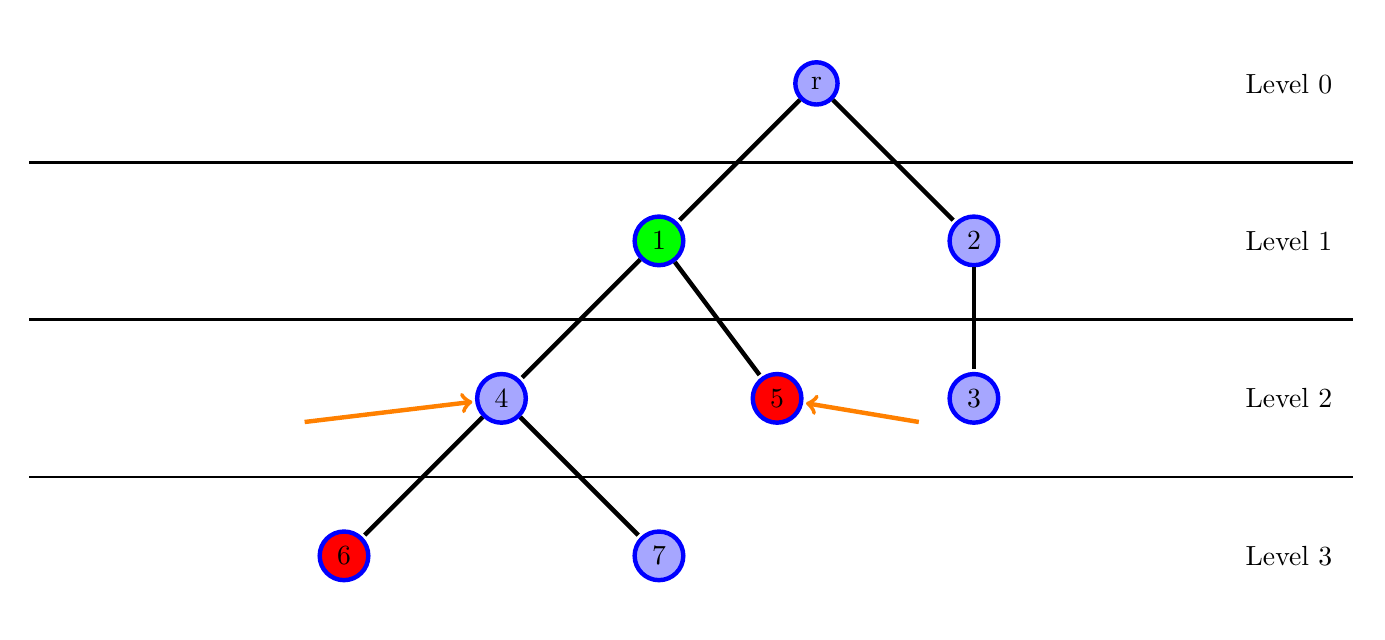
\begin{tikzpicture}[shorten >=1pt, auto, node distance=3cm, ultra thick]
   \node[circle] at (6,0) {{Level 0}};
   \node[circle] at (6,-2) {{Level 1}};
   \node[circle] at (6,-4) {{Level 2}};
   \node[circle] at (6,-6) {{Level 3}};
   \draw (-10,-1) -- (6.85,-1) [line width=1.0pt];
   \draw (-10,-3) -- (6.85,-3) [line width=1.0pt];
   \draw (-10,-5) -- (6.85,-5) [line width=1.0pt];
   \begin{scope}[every node/.style={circle,draw=blue,fill=blue!35!}]
    \node (v1) at (0,0) {r};
    \node (v2) at (-2, -2) [fill=green] {1};
    \node (v3) at (2, -2) {2};
    \node (v4) at (2, -4) {3};
    \node (v5) at (-4, -4) {4};
    \node (v6) at (-0.5, -4) [fill=red] {5};
    \node (v7) at (-6, -6) [fill=red] {6};
    \node (v8) at (-2, -6) {7};
   \end{scope}
   \begin{scope}[every edge/.style={draw=black,ultra thick}]
    \draw  (v1) edge node{} (v2);
    \draw  (v1) edge node{} (v3);
    \draw  (v2) edge node{} (v5);
    \draw  (v2) edge node{} (v6);
    \draw  (v3) edge node{} (v4);
    \draw  (v5) edge node{} (v7);
    \draw  (v5) edge node{} (v8);
   \end{scope}
   \draw (-6.5,-4.3) edge [->, orange] node{} (v5);
   \draw (1.3, -4.3) edge [->, orange] node{} (v6);
\end{tikzpicture}
\end{figure}
\newpage
\noindent
At this point, we move them both up \emph{simultaneously} until they converge. Eventually they will converge and the node that they converge on will be the lowest common ancestor.
\begin{figure}[!ht]
\caption{Then, we move them up simultaneously until they converge. The node they converge on is the lowest common ancestor.}
\centering
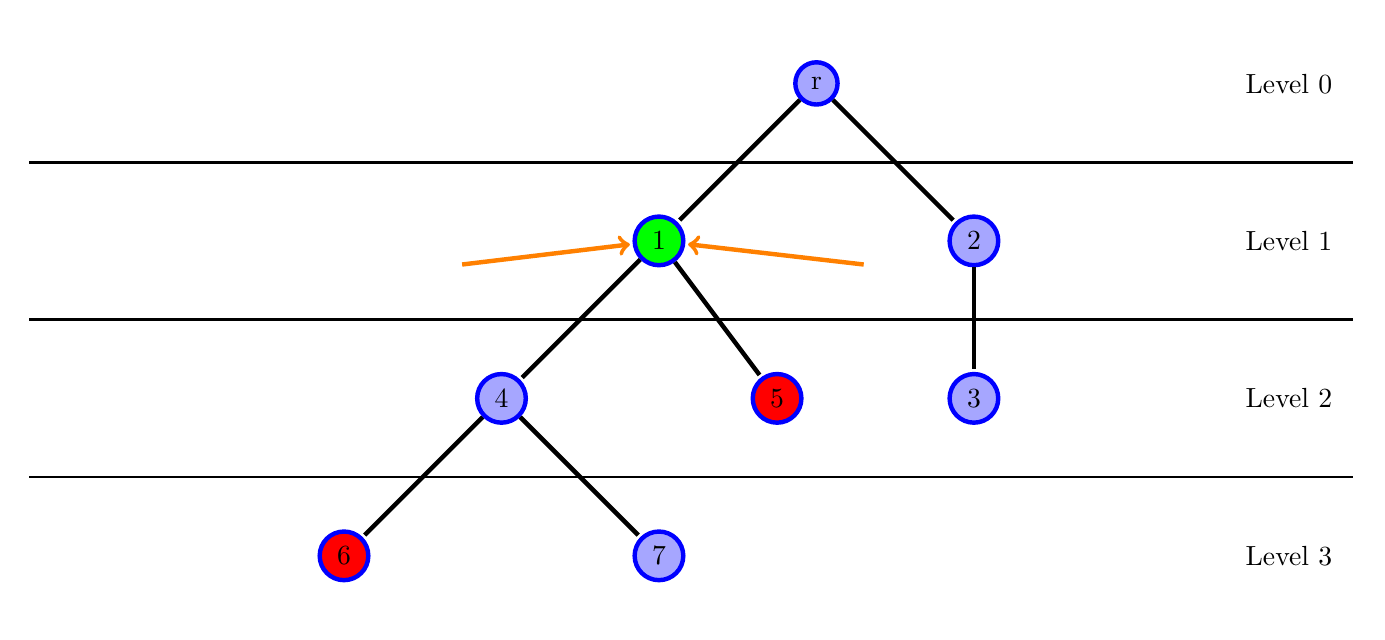
\begin{tikzpicture}[shorten >=1pt, auto, node distance=3cm, ultra thick]
   \node[circle] at (6,0) {{Level 0}};
   \node[circle] at (6,-2) {{Level 1}};
   \node[circle] at (6,-4) {{Level 2}};
   \node[circle] at (6,-6) {{Level 3}};
   \draw (-10,-1) -- (6.85,-1) [line width=1.0pt];
   \draw (-10,-3) -- (6.85,-3) [line width=1.0pt];
   \draw (-10,-5) -- (6.85,-5) [line width=1.0pt];
   \begin{scope}[every node/.style={circle,draw=blue,fill=blue!35!}]
    \node (v1) at (0,0) {r};
    \node (v2) at (-2, -2) [fill=green] {1};
    \node (v3) at (2, -2) {2};
    \node (v4) at (2, -4) {3};
    \node (v5) at (-4, -4) {4};
    \node (v6) at (-0.5, -4) [fill=red] {5};
    \node (v7) at (-6, -6) [fill=red] {6};
    \node (v8) at (-2, -6) {7};
   \end{scope}
   \begin{scope}[every edge/.style={draw=black,ultra thick}]
    \draw  (v1) edge node{} (v2);
    \draw  (v1) edge node{} (v3);
    \draw  (v2) edge node{} (v5);
    \draw  (v2) edge node{} (v6);
    \draw  (v3) edge node{} (v4);
    \draw  (v5) edge node{} (v7);
    \draw  (v5) edge node{} (v8);
   \end{scope}
   \draw (-4.5,-2.3) edge [->, orange] node{} (v2);
   \draw (0.6, -2.3) edge [->, orange] node{} (v2);
\end{tikzpicture}
\end{figure}
\\
\noindent
And here is code that does it:
\begin{lstlisting}
//....assuming the rooted tree code above
int lca(int x, int y) {
	//find lowest pointer
	//actually, we just make sure `x' is the lowest
	//(Lowest in the tree ---> highest level)
	if (level[x] < level[y]) {
		int temp = x;
		x = y;
		y = temp;
	}
	//move the lowest up until same level
	while (level[x] != level[y]) {
		x = parent[x];
	}
	//move both up simultaneously until
	//they converge
	while (x != y) {
		x = parent[x];
		y = parent[y];
	}
	//x and y both point to LCA
	return x;
}
\end{lstlisting}
If $h$ is the height of the tree, the runtime of this algorithm is $\boxed{O(h)}$.
\subsection{Square-Root Decomposition}
We can actually use the square-root decomposition method to solve the LCA problem. This won't be covered in these lecture notes (it's not very fast).
\subsection{Binary Lifting (Sparse Table DP)}
Refer to the lecture notes on dynamic programming. This is the best way to answer the LCA query (in terms of run-time vs. time to code).
\subsection{Reduction to Range Minimum Query}
The algorithms developed above are pretty good, but they're not the best we can do. You may have noticed that we didn't really take advantage of pre-computation like we did for other solutions to query problems. Our goal for this section is to devise some data structure that we can pre-compute that will help us answer LCA queries quickly. More specifically, we're going to figure out a way to turn an LCA query into a RMQ (range minimum query) which, as we saw in the set of lecture notes on array data structures, can be answered in $O(\log{N})$. The construction of the following algorithm is far from obvious, so just try and follow along without worrying too much about how it was derived.
\\\\
\noindent
Imagine you're manually performing a depth-first search on a tree, tracing the order that DFS visits each node without picking up your finger. We maintain a {\bf{list}}, denoted `euler[]'. Every time you move into a node, add it to the end of `euler[]' (including nodes that you backtrack to). Consider the following example:
\begin{figure}[!ht]
\caption{An example tree.}
\centering
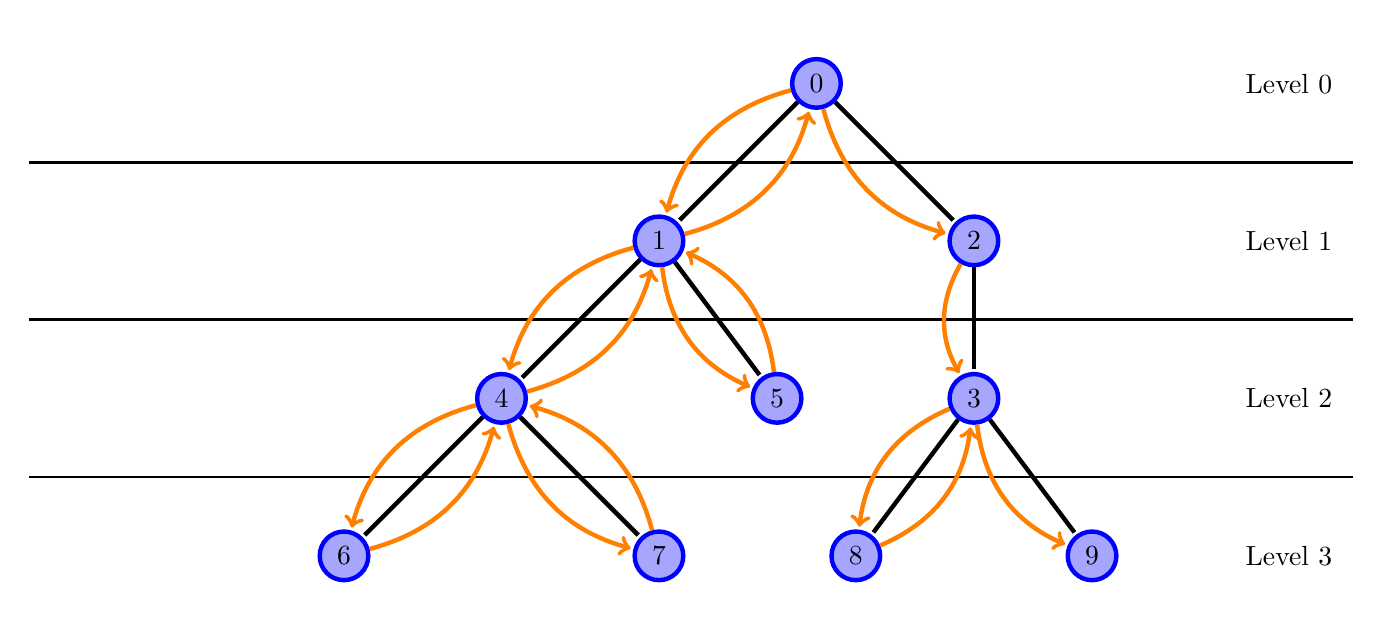
\begin{tikzpicture}[shorten >=1pt, auto, node distance=3cm, ultra thick]
   \node[circle] at (6,0) {{Level 0}};
   \node[circle] at (6,-2) {{Level 1}};
   \node[circle] at (6,-4) {{Level 2}};
   \node[circle] at (6,-6) {{Level 3}};
   \draw (-10,-1) -- (6.85,-1) [line width=1.0pt];
   \draw (-10,-3) -- (6.85,-3) [line width=1.0pt];
   \draw (-10,-5) -- (6.85,-5) [line width=1.0pt];
   \begin{scope}[every node/.style={circle,draw=blue,fill=blue!35!}]
    \node (v1) at (0,0) {0};
    \node (v2) at (-2, -2) {1};
    \node (v3) at (2, -2) {2};
    \node (v4) at (2, -4) {3};
    \node (v5) at (-4, -4) {4};
    \node (v6) at (-0.5, -4) {5};
    \node (v7) at (-6, -6) {6};
    \node (v8) at (-2, -6) {7};
    \node (v9) at (0.5, -6) {8};
    \node (v10) at (3.5, -6) {9};
   \end{scope}
   \begin{scope}[every edge/.style={draw=black,ultra thick}]
    \draw  (v1) edge node{} (v2);
    \draw  (v1) edge node{} (v3);
    \draw  (v2) edge node{} (v5);
    \draw  (v2) edge node{} (v6);
    \draw  (v3) edge node{} (v4);
    \draw  (v5) edge node{} (v7);
    \draw  (v5) edge node{} (v8);
    \draw  (v4) edge node{} (v9);
    \draw  (v4) edge node{} (v10);
   \end{scope}
   \begin{scope}[->, every edge/.style={draw=black,ultra thick}]
    \draw  (v1) edge [bend right, orange] node{} (v2);
    \draw  (v2) edge [bend right, orange] node{} (v5);
    \draw  (v5) edge [bend right, orange] node{} (v7);
    \draw  (v7) edge [bend right, orange] node{} (v5);
    \draw  (v5) edge [bend right, orange] node{} (v8);
    \draw  (v8) edge [bend right, orange] node{} (v5);
    \draw  (v5) edge [bend right, orange] node{} (v2);
    \draw  (v2) edge [bend right, orange] node{} (v6);
    \draw  (v6) edge [bend right, orange] node{} (v2);
    \draw  (v2) edge [bend right, orange] node{} (v1);
    \draw  (v1) edge [bend right, orange] node{} (v3);
    \draw  (v3) edge [bend right, orange] node{} (v4);
    \draw  (v4) edge [bend right, orange] node{} (v9);
    \draw  (v9) edge [bend right, orange] node{} (v4);
    \draw  (v4) edge [bend right, orange] node{} (v10);
   \end{scope}
\end{tikzpicture}
\end{figure}
\begin{table}[!ht]
\centering
\caption{One possible `euler[]' list for the tree above. Note that there can be others, depending on the order the DFS call visits the nodes.}
\label{my-label}
\begin{tabular}{l|c|l|c|c|c|c|c|c|c|c|l|l|l|l|l|l|}
\cline{2-17}
euler{[}{]} = & 0 & 1 & 4 & 6 & 4 & 7 & 4 & 1 & 5 & 1 & 0 & 2 & 3 & 8 & 3 & 9 \\ \cline{2-17} 
level{[}{]} = & 0 & 1 & 2 & 3 & 2 & 3 & 2 & 1 & 2 & 1 & 0 & 1 & 2 & 3 & 2 & 3 \\ \cline{2-17} 
\end{tabular}
\end{table}
\newpage
\noindent
We also included a different `level[]' array --- level[i] is just the level that node euler[i] is on. With both of these arrays, we're going to answer LCA queries. Let's go through a couple examples:
\\\\
$\boxed{\text{Example 1 - LCA(7, 5) = 1}}$
\\\\
First find node $5$ and node $7$ in the `euler[]' list. Notice how the answer, LCA(7, 5) = 1, is the node with the \emph{lowest} level number between nodes $7$ and $5$ in `euler[]'.
\begin{table}[!ht]
\centering
%\caption{}
\label{my-label}
\begin{tabular}{l|c|l|c|c|c|
>{\columncolor[HTML]{009901}}c |
>{\columncolor[HTML]{009901}}c |
>{\columncolor[HTML]{34CDF9}}c |
>{\columncolor[HTML]{009901}}c |c|l|l|l|l|l|l|}
\cline{2-17}
euler{[}{]} = & 0 & 1 & 4 & 6 & 4 & 7 & 4 & 1 & 5 & 1 & 0 & 2 & 3 & 8 & 3 & 9 \\ \cline{2-17} 
level{[}{]} = & 0 & 1 & 2 & 3 & 2 & 3 & 2 & 1 & 2 & 1 & 0 & 1 & 2 & 3 & 2 & 3 \\ \cline{2-17} 
\end{tabular}
\end{table}
\\
In general, we get the following observation:
$${\emph{LCA(u, v) = the node with the lowest level number between nodes $u$ and $v$ in the `euler[]' list.}}$$
$\boxed{\text{Example 2 - LCA(4, 3) = 0}}$
\\\\
We have a similar situation here, except notice how there are multiple occurrences of both $3$ and $4$ inside `euler[]'. It actually turns out that it doesn't really matter which one we choose, and so we'll always choose the first (from left to right) occurrence. Again, the answer of $0$ is indeed the lowest leveled node between $4$ and $3$.
\begin{table}[!ht]
\centering
%\caption{}
\label{my-label}
\begin{tabular}{l|c|l|
>{\columncolor[HTML]{009901}}c |
>{\columncolor[HTML]{009901}}c |
>{\columncolor[HTML]{009901}}c |
>{\columncolor[HTML]{009901}}c |
>{\columncolor[HTML]{009901}}c |
>{\columncolor[HTML]{009901}}c |
>{\columncolor[HTML]{009901}}c |
>{\columncolor[HTML]{009901}}c |
>{\columncolor[HTML]{34CDF9}}l |
>{\columncolor[HTML]{009901}}l |
>{\columncolor[HTML]{009901}}l |l|l|l|}
\cline{2-17}
euler{[}{]} = & 0 & 1 & 4 & 6 & 4 & 7 & 4 & 1 & 5 & 1 & 0 & 2 & 3 & 8 & 3 & 9 \\ \cline{2-17} 
level{[}{]} = & 0 & 1 & 2 & 3 & 2 & 3 & 2 & 1 & 2 & 1 & 0 & 1 & 2 & 3 & 2 & 3 \\ \cline{2-17} 
\end{tabular}
\end{table}
\\
Intuitively, all of the nodes between $u$ and $v$ in `euler[]' give us a path from $u$ to $v$ (although some nodes appear more than once, but we ignore that). One important fact, which is not very hard to agree with, is that the LCA of two nodes is \emph{always} on the path (remember that there is only one path between two nodes) between them. We can actually take this a step further and say that the LCA is the highest node (lowest `level[]' value) on the path between $u$ and $v$ --- drawing a few examples should show that this is correct. \\\\
We get the following algorithm:
\\\\
(1) Pre-compute the `euler[]' and `level[]' arrays. Additionally, we need the array `first\_occurrence[node]' which gives us the index of the \emph{first occurrence} of `node' in `euler[]'. \\
(2) Suppose RMQ(i, j, level) gives us the index of the smallest element between $i$ and $j$ in `level[]'. Then, we can answer LCA queries with the following formula:
$$\boxed{\text{LCA(u, v) = euler[RMQ(first\_occurence[i], first\_occurence[j], level)];}}$$
\newpage
\noindent
Here is code which does just that --- all we're doing is computing all of this information in one DFS of the tree. Notice how similar it is to the DFS we used at the beginning to calculate `parent[]' and `level[]'. 
\begin{lstlisting}
//initialize adjacency list
ArrayList[] adj_list = new ArrayList[n];
for (int i = 0; i < n; i++)
	adj_list[i] = new ArrayList();
//read in the edges (there are n-1 of them *ALWAYS*)
for (int i = 0; i < (n-1); i++) {
	int from = readInt();
	int to = readInt();
	adj_list[from].add(to);
	adj_list[to].add(from);
}
//read root
int root = readInt();
//the most amount of nodes in the euler[]/level[] list is 2*n+1
int[] euler = new int[2*n+1];
int[] level = new int[2*n+1];
//stores the first_occurrence of each node...
int[] first_occurrence = new int[n];
//initialize first_occurrence to all -1s, indicating
//that they havent been set yet
Arrays.fill(first_occurrence, -1);

//euler_counter will allow us to append to the euler list
int euler_counter = 0;
//fill in these three arrays with one dfs call
dfs(root, -1, 0);

//precomputes level[], euler[], and first_occurrence[]
void dfs(int cur_node, int prev_node, int cur_level) {
	//we just came into a node, add it to euler[]
	euler[euler_counter] = cur_node;
	//add the level corresponding to this node
	level[euler_counter] = cur_level;
	//if first occurrence of this node hasn't been assigned,
	//assign it.
	if (first_occurrence[cur_node] == -1) {
		first_occurrence[cur_node] = euler_counter;
	}
	//increment euler counter
	euler_counter++;
	for (int neighbor : adj_list[cur_node]) {
		//don't want to jump back up
		if (neighbor == prev_node) continue;
		//go into this node
		dfs(neighbor, cur_node, cur_level + 1);
		//now we just came out of this node, so we append `cur_node'
		//to euler[]
		euler[euler_counter] = cur_node;
		level[euler_counter] = cur_level;
		euler_counter++;
	}
}

//compute rmq
int rmq(int i, int j) {
	//make sure i < j
	if (i > j) {
		int temp = i;
		i = j;
		j = temp;
	}
	//return the index with the lowest level[]
	//between [i, j]
	//USE CODE THAT WE DEVELOPED IN
	//ARRAY DATASTRUCTURES LECTURE NOTES
	//segment tree, sqrt decomposition, etc...
}

//compute the lca of u and v. exactly as we described above
int lca(int u, int v) {
	int from = first_occurrence[u];
	int to = first_occurrence[v];
	int idxOf = rmq(from, to);
	return euler[idxOf];
}
\end{lstlisting}
The runtime of this algorithm depends on how fast you can implement the RMQ operation. The fastest we can do for that is $O(\lg n)$. However, we also have to account for the preprocessing step. Recall that a DFS takes $O(V+E)$ where $V$ and $E$ are the number of nodes and edges in the graph. If we use the fact that, for trees, $E = V-1$, we get $O(V+E) = O(V+V-1) = O(2V - 1) = O(V) = O(n)$. In summary,
\begin{center}
\fbox{\begin{minipage}{11.339em}
Pre-processing time: $O(n)$\\
\hspace{-15mm}Query time: $O(\log n)$
\end{minipage}
}
\end{center}
\section{Path Sum Queries}
Now we turn to another query problem on trees: the path sum query. Suppose we're given an (unrooted) tree where each edge is assigned a weight. We define the sum query as\\
$$\boxed{\text{sum($x$, $y$)} = \text{the sum of the edge weights on the unique path from $x$ to $y$}}$$
\begin{figure}[!ht]
\caption{An example (unrooted) tree with weights assigned to edges.}
\centering
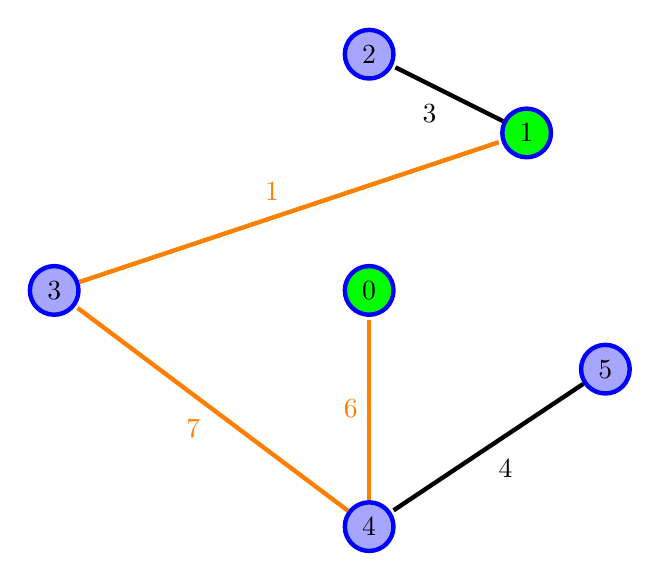
\begin{tikzpicture}[shorten >=1pt, auto, node distance=3cm, ultra thick]
   \begin{scope}[every node/.style={circle,draw=blue,fill=blue!35!}]
    \node (v1) at (0,0) [fill=green] {0};
    \node (v2) at (2, 2) [fill=green] {1};
    \node (v3) at (0, 3) {2};
    \node (v4) at (-4, 0) {3};
    \node (v5) at (0, -3) {4};
    \node (v6) at (3, -1) {5};
   \end{scope}
   \begin{scope}[every edge/.style={draw=black,ultra thick}]
    \draw  (v2) edge node{3} (v3);
    \draw  (v5) edge [orange] node {7} (v4);
    \draw  (v6) edge node{4} (v5);
    \draw  (v5) edge [orange] node{6} (v1);
    \draw  (v4) edge [orange] node{1} (v2);
   \end{scope}
\end{tikzpicture}
\end{figure}
\newpage
\noindent
For example, in the tree above we have $\boxed{\text{sum($0$, $1$)} = 6 + 7 + 1 + 3 = 17}$. How can we support this operation as quickly as possible?
\\\\
\noindent
TODO: Finish this.

\section{Heavy-Light Decomposition}
TODO: Soon.
\section{Building a Segment Tree on a Tree}
TODO: (Maybe)
\section{Centroid Decomposition}
TODO: Soon.
\section{DP on a Tree}
Refer to the lecture notes on dynamic programming.
\section{Comments}
In this set of lecture notes we took a look at a couple of different problems and solutions to those problems. At the heart of many tree problems is the notion of the \emph{lowest common ancestor} of two nodes. It's important to note that the LCA of two nodes is only defined for rooted trees. There are four popular methods to find the LCA of two nodes in a rooted tree: the naive method, square-root decomposition, the binary lifting method, and using a reduction to RMQ --- the last two being the best. We then delved into the path sum query problem and leveraged the notion of \emph{rooting} a tree so that the LCA becomes well defined, and then used it to answer path sum queries. If we introduce the edge-update operation, that solution breaks completely and we must resort to using heavy-light decomposition or centroid decomposition. While the list of material covered here is not exhaustive, hopefully you are now comfortable with the basic techniques used on trees.
\section{Problems}
$$\boxed{\text{http://www.spoj.com/problems/LCASQ/}}$$
$$\boxed{\text{https://open.kattis.com/problems/tourists}}$$
\section*{Code Appendix}
\subsection*{RMQ Code}
This uses square-root decomposition to solve the RMQ problem. You may use it with the LCA reduction method. Pre-processing time is $O(n)$ and query time is $O(\sqrt{n})$.
\begin {lstlisting}
class RMQ {
	int[] array;
	int[] sqrt;

	RMQ(int[] array) {
		this.array = array;
		int sq = (int) Math.ceil(Math.sqrt(array.length));
		this.sqrt = new int[sq+1];
		int j = 0;
		for (int i = 0; i < array.length; i += sq, j++) {
			int end = Math.min(array.length-1, i+sq-1);
			int min = Integer.MAX_VALUE;
			int minIdx = -1;
			for (int k = i; k <= end; k++) {
				if (array[k] < min) {
					min = array[k];
					minIdx = k;
				}
			}
			sqrt[j] = minIdx;
		}
	}

	int query(int l, int r) {
		int sq = (int)  Math.ceil(Math.sqrt(array.length));
		int j = 0;
		int min = Integer.MAX_VALUE;
		int minIdx = -1;
		for (int i = 0; i < array.length; i += sq, j++) {
			int lo = i;
			int hi = i+sq-1;
			if (lo >= l && hi <= r) {
				int idx = sqrt[j];
				if (array[idx] < min) {
					min = array[idx];
					minIdx = idx;
				}
			} else {
				int x=-1, y=-1;
				if (l >= lo && r > hi) {
					x = l;
					y = r;
				} else if (r <= hi && l < lo) {
					x = lo;
					y = r;
				} else if (l >= lo && r <= hi) {
					x = l;
					y = r;
				}
				if (x != -1 && y != -1) {
					for (int k = x; k <= y; k++) {
						if (array[k] < min) {
							min = array[k];
							minIdx = k;
						}
					}
				}
			}
		}
		return minIdx;
	}
}
\end{lstlisting}
\subsection*{Binary Lifting Code}
Takes $O(n \log n)$ pre-processing and $O(\log n)$ per query.
\begin{lstlisting}
class LCA {
	
	//dp[i][j] = node i's 2^jth parent
	int[][] dp;
	int[] parent, level;
	int N;
	//parent[root] = root
	//parent[x] = parent of x when the tree is rooted at root
	//level[root] = 0
	//level[x] = distance from root to x
	public LCA(int[] parent, int[] level) {
		N = parent.length;
		this.parent = parent;
		this.level = level;
		precompute();
	}
	
	public void precompute() {
		int log = 0;
		while (1<<log <= N) log++;

		dp = new int[N][log];
		for (int i = 0; i < N; i++) {
			for (int j = 0; j < log; j++) {
				dp[i][j] = -1;
			}
		}
		for (int i = 0; i < N; i++) {
			dp[i][0] = parent[i];
		}
		for (int j = 1; (1<<j)<N; j++) {
			for (int i = 0; i < N; i++) {
				if (dp[i][j-1] != -1) {
					dp[i][j] = dp[dp[i][j-1]][j-1];
				}	
			}
		}
	}

	public int lca(int u, int v) {
		if (level[u] < level[v]) {
			int temp = v;
			v = u;
			u = temp;
		}
		int log = 1;
		while ((1<<log)<=level[u]) log++;
		log--;
		for (int i = log; i >= 0; i--) {
			if (level[dp[u][i]] >= level[v]) {
				u = dp[u][i];
			}
		}
		if (u == v) return u;
		for (int i = log; i >= 0; i--) {
			if (dp[u][i] != -1 && dp[u][i] != dp[v][i]) {
				u = dp[u][i];
				v = dp[v][i];
			}
		}
		return parent[u];
	}
}
\end{lstlisting}
\end{document}
